\documentclass[a4paper]{article}

%% Language and font encodings
\usepackage[english]{babel}
\usepackage[utf8x]{inputenc}
\usepackage[T1]{fontenc}
\usepackage{graphicx}
\usepackage{caption}
\usepackage{subcaption}
\usepackage{eurosym}
\usepackage{multirow}
\usepackage{footnote}
\usepackage{listings}
\usepackage{color}
\usepackage{pdfpages}
\usepackage{listings}
\renewcommand{\ttdefault}{pcr}


\lstset{
  breaklines=true,
  postbreak=\mbox{\textcolor{red}{$\hookrightarrow$}\space},
  %basicstyle=\ttfamily,
  columns=fixed,
  %keepspaces=true,
}


%% Sets page size and margins
\usepackage[a4paper,top=3cm,bottom=2cm,left=3cm,right=3cm,marginparwidth=1.75cm]{geometry}

%% Useful packages
\usepackage{amsmath}
\usepackage{graphicx}
\usepackage[colorinlistoftodos]{todonotes}
\usepackage[colorlinks=true, allcolors=blue]{hyperref}
\begin{document}

\begin{titlepage}

\newcommand{\HRule}{\rule{\linewidth}{0.5mm}} % Defines a new command for the horizontal lines, change thickness here

\center % Center everything on the page
 
%----------------------------------------------------------------------------------------
%	HEADING SECTIONS
%----------------------------------------------------------------------------------------

\textsc{\LARGE Ecole Polytechnique de Bruxelles}\\[1.5cm] % Name of your university/college
\textsc{\LARGE University of Leeds}\\[1.5cm]
\textsc{\large Johnston Lab Internship}\\[0.5cm] % Minor heading such as course title

%----------------------------------------------------------------------------------------
%	TITLE SECTION
%----------------------------------------------------------------------------------------

\HRule \\[0.4cm]
{ \huge \bfseries Technical description and User guide: Devices Synchronization using Arduino MEGA controller as I2C master for data integration in tiff files}\\[0.4cm] % Title of your document
\HRule \\[1.5cm]
 
%----------------------------------------------------------------------------------------
%	AUTHOR SECTION
%----------------------------------------------------------------------------------------

\begin{minipage}{0.4\textwidth}
\begin{flushleft} \large
\emph{Author:}\\
Maxime \textsc{Verstraeten} % Your name
\end{flushleft}
\end{minipage}
~
\begin{minipage}{0.4\textwidth}
\begin{flushright} \large
\emph{Supervisor:} \\
Jamie \textsc{Johnston}\\[0.3cm] % Supervisor's Name
\end{flushright}
\end{minipage}\\[2cm]

% If you don't want a supervisor, uncomment the two lines below and remove the section above
%\Large \emph{Author:}\\
%John \textsc{Smith}\\[3cm] % Your name

%----------------------------------------------------------------------------------------
%	DATE SECTION
%----------------------------------------------------------------------------------------

{\large \today}\\[2cm] % Date, change the \today to a set date if you want to be precise

%----------------------------------------------------------------------------------------

\vfill % Fill the rest of the page with whitespace

\end{titlepage}


\noindent\rule{\textwidth}{1pt}

\tableofcontents

\newpage

\listoffigures

\newpage



\section{Introduction}
This user guide intends to provide the user with the information required to use and understand the synchronization device developed at JohnstonLab as well as giving some clues regarding troubleshooting.\\

This device was developed as part of my internship at JohnstonLab (Leeds University, UK) during my master's years as a student engineer from the Université Libre de Bruxelles, Belgium.

This device is part of the rig that allows the lab to perform in-vivo measurements and experiments on mice. This device gathers data from other devices around the lab (lick-sensor, thermography camera, motion sensors, strain gauges, ...) and allows to synchronize them before sending the values to a computer over I2C and plot the values.\\

Note: The workflow, thoughts, issues, ... for this project are discussed in my OneNote.\\

The latest software and documentation updates are available on my Github: \url{https://github.com/maverstr/i2cAurora}

\section{Objective}
This device gathers from different experimental devices, either digital or analog signals, through different BNC connectors and some PS/2 connectors. 
It then is able to plot them in a user-friendly interface using Arduino Serial plotter to easily keep an eye on all the signals.

It also acts as an I2C master device to transmit data through ScanImage (\url{http://scanimage.vidriotechnologies.com/display/SI2015/I2C+data+recording}) which emulates an I2C slave on the computer.
ScanImage can then interpret this I2C Data and put it in the description of tiff files for each frame.

This allows to have every signal values inside each frame metadata.

The µC also gets data from two optical mice that act as a motion sensor and does the computation for the path taken by the mouse.

\section{Hardware}

\begin{figure}[h!]
    \centering
    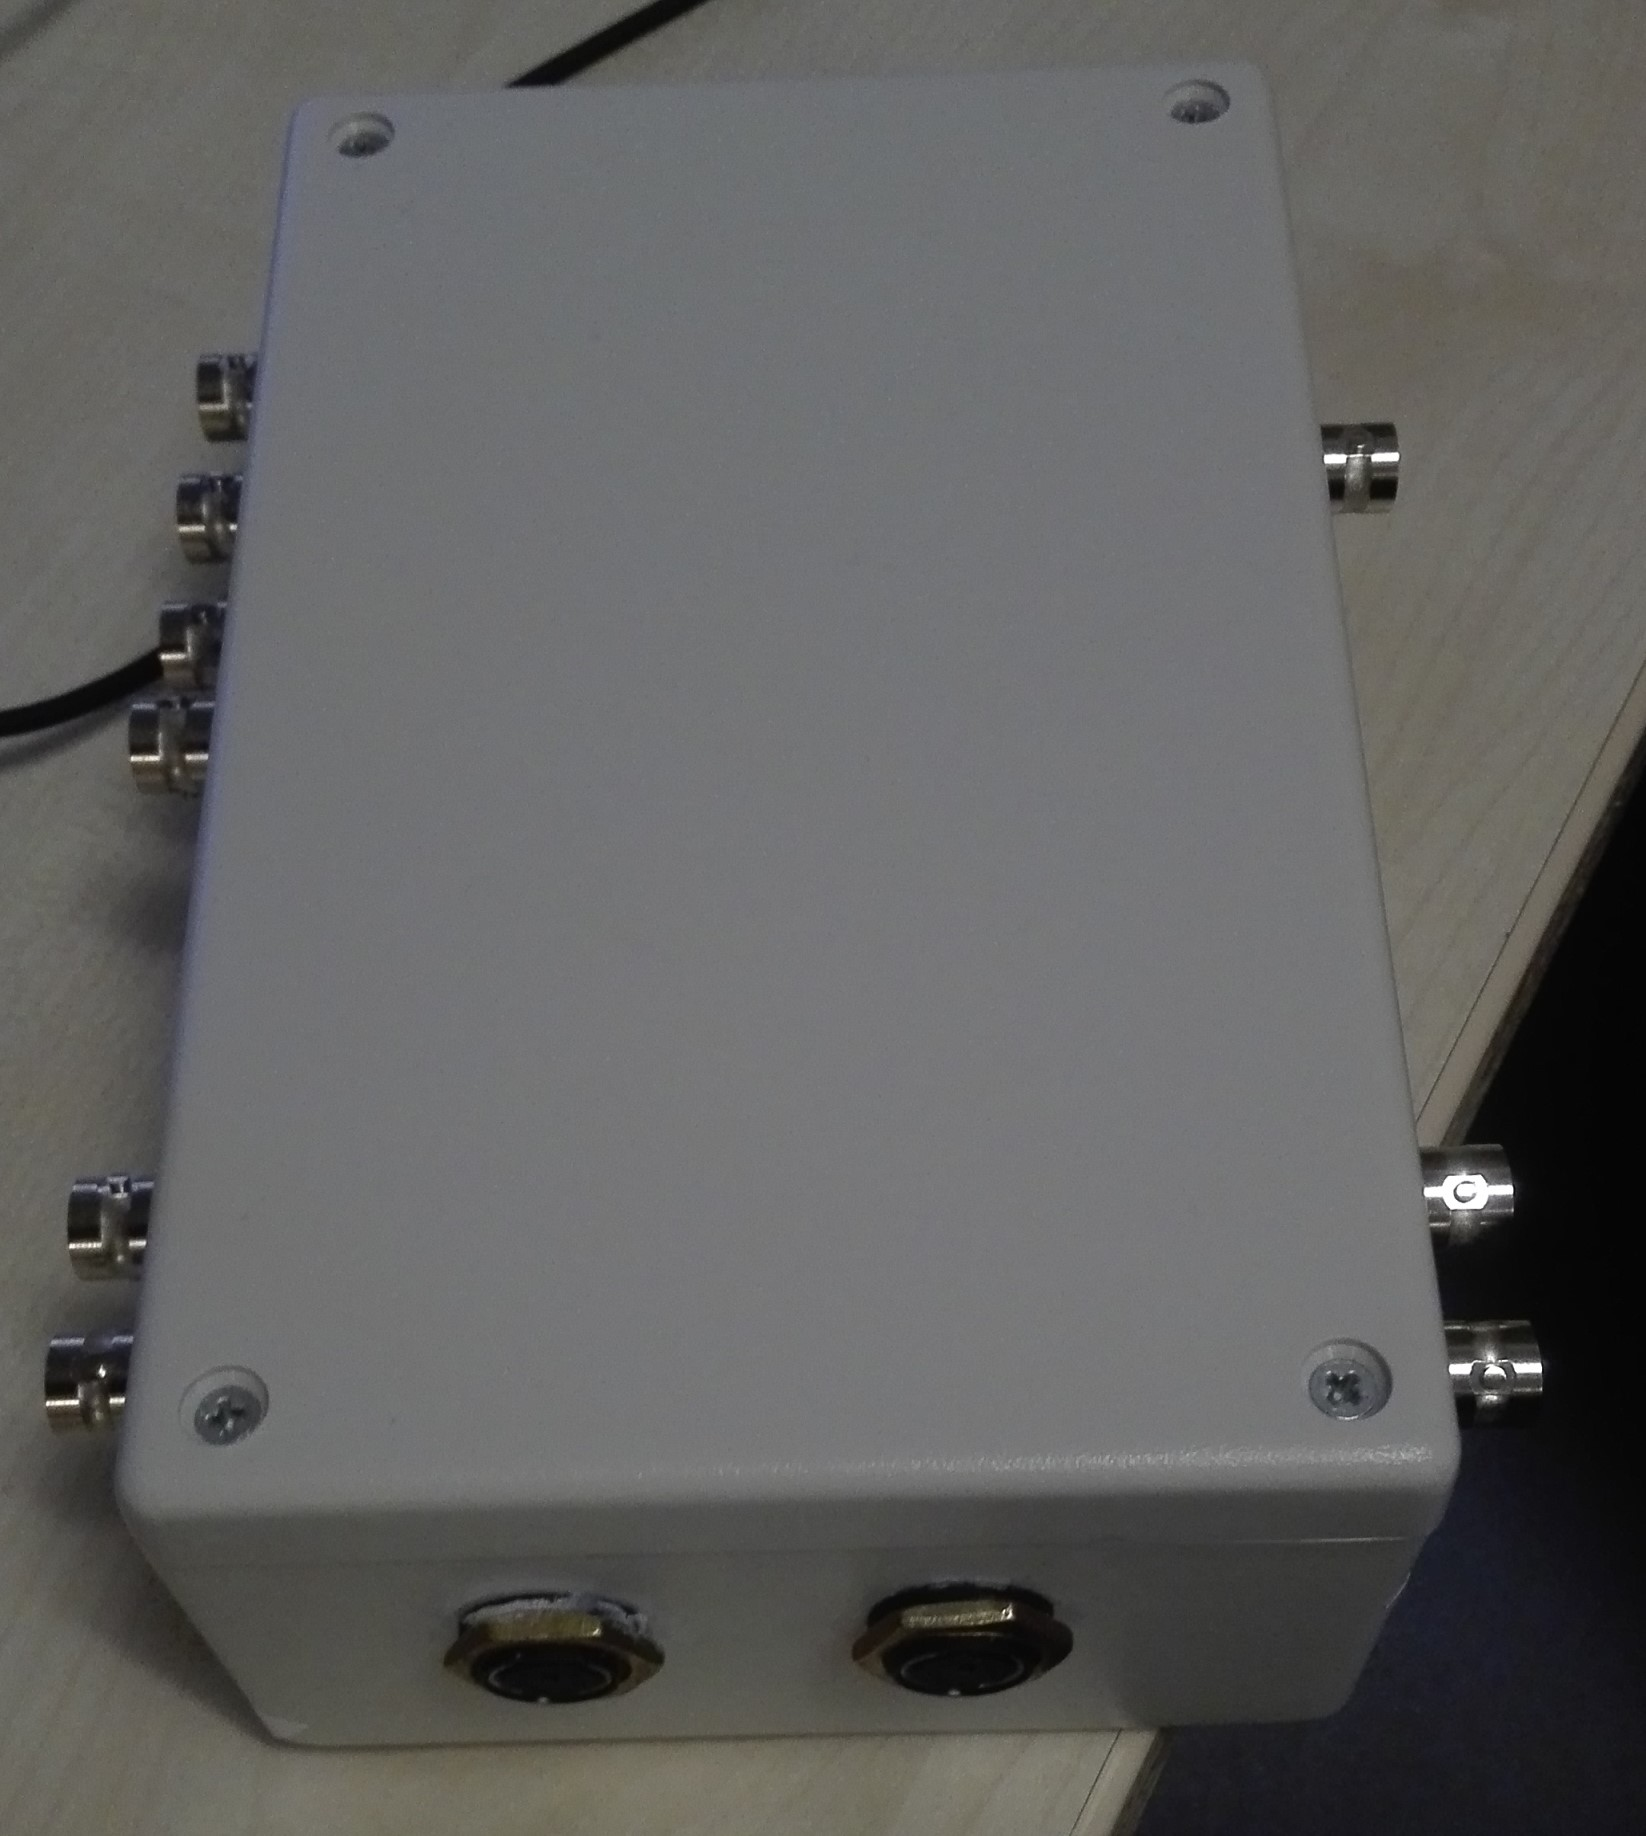
\includegraphics[width = 6cm]{images/synchroBox.jpg}
    \caption{Synchronization box}
    \label{fig:synchroBox}
\end{figure}

\subsection{Arduino MEGA}
The µC is the Arduino MEGA, chosen for the high number of analog and digital inputs as well as easy configuration and user-friendly plotting.


\subsection{Enclosure}
The enclosure contains the µC and hold it in place for simple manipulations. The enclosure also comes with 16 BNC holes and 2 PS/2 holes.
The enclosure is chosen from RS: \url{https://uk.rs-online.com/web/p/general-purpose-enclosures/3815164/} and CAD designed for documentation purpose and easy hole drilling.

\begin{figure}[h!t!b!]
    \centering
        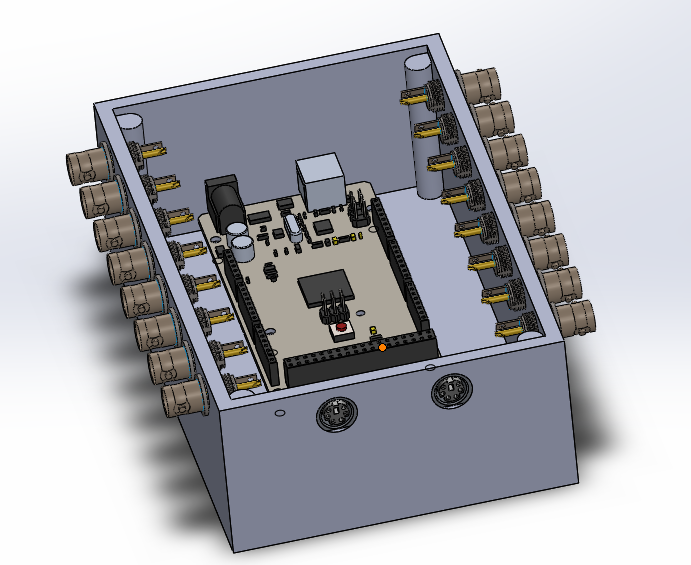
\includegraphics[width = 10cm]{images/enclosure.PNG}
    \caption{CAD View of the enclosure}
    \label{fig:enclosure1}
\end{figure}

\begin{figure}[h!t!b!]
    \centering
        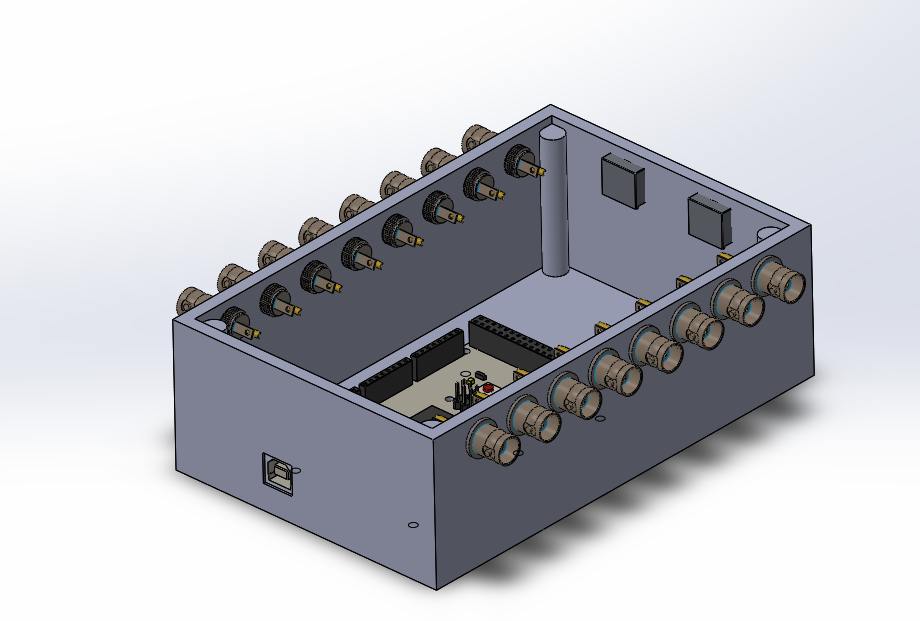
\includegraphics[width = 10cm]{images/enclosure2.PNG}
    \caption{CAD View of the enclosure}
    \label{fig:enclosure2}
\end{figure}

The Plans for drilling holes are presented in appendix \ref{plans} and are available on scale 1:1 on demand.
The box can be seen on Figure \ref{fig:synchroBox}.


\subsection{Connectors}
The connectors used to transmit data are BNC connectors. This is actually not the best option but the more practical to use as everything in the lab presents BNC connectors and BNC cables.

There are also 2 PS/2 connectors used for the motion sensor using optical mice which communicates using PS/2.

\newpage
\section{Software}
The µC is programmed using the Arduino IDE.
The code is quite simple and comes in a few main parts:
\subsection{Motion sensor acquisition and computation}
Using the developed libraries, the µC receives data from 2 optical mice and compute the path taken by a running mouse on a ball.
This is all done in the additional .h and .cpp libraries.
\begin{lstlisting}[language=C++]
#include "MotionSensorAcq.h"
\end{lstlisting}

The mice are setup on setup part using "motionSensorSetup()" with defined clock and data pins in variable definition. Then the data is acquired using
\begin{lstlisting}[language=C++]
motionSensorAcq(&motionSensorValuesArray[0]);
\end{lstlisting}
which basically inserts the data into the pointed array.

\subsection{Other data acquisition}
The rest of the incoming data from other devices are simply processed using Arduino digital or analog read functions. Some data like the strain gauge are just re-scaled to proper values.

\subsection{Plotting}
The plotting is easily done by following the guidelines for Arduino Serial plotter. Basically, the Arduino serial plotter regularly reads the serial buffer and interprets the data. This obviously works only as long as the data are correctly sent to the serial buffer. 

\subsection{I2C Communication}
The integers value are first casted into String to be able to use the .toCharArray on them to form char arrays which can then be transmitted over I2C.
The transmission itself is done using the Wire library.

\subsection{I2C Slave}
ScanImage acts as an I2C slave and is handled by MATLAB. This part will not be discussed here but is explained in the relevant documentation (\url{http://scanimage.vidriotechnologies.com/display/SI2015/I2C+data+recording}).

\section{How to use?}
Simply plug the connectors to the corresponding pins (or change them in the declaration part of the code).
BNC connectors have names on the lab device for pins connections. For your own device, feel free to change the pins to your desire.\\

If the optical mice motion sensor are not plugged in (or malfunctioning for whatever reason), make sure that 
\begin{lstlisting}
#define MOTION_SENSOR
\end{lstlisting}
IS commented. 
If the optical mice are plugged in and working, and you want to use them, remove any "//" in front of that line to activate the relevant parts of the code. You need to recompile and upload the code to the µC for the change to take effect.\\

Use USB to power the Arduino and allow Serial communication to go through. Open the Serial Plotter using tools in Arduino IDE. You should see the relevant signal on the window.
Note: the Serial rate is set to 500 000 bauds to allow fast communication of multiple signals at high sampling rate. You have to set the Serial Monitor and Plotter to this value.

The values are automatically sent over I2C when triggered externally by the Labjack. If you want constant I2C communication without requiring a trigger, overwrite cameraTriggerValue to 1 (compile and upload the code to the µC for the change to take effect). Note that this may have unexpected results. 

\section{Expected Results}
When using the Serial plotter, the window should show the relevant signals in different colors (see Figure \ref{fig:plotting} where respiration signal (human) is in red, optical mice X, Y, Z in reddish, blue and green and yellow here is a copy from red simulating the i2C scaling of the value.
Other devices are not connected.).

\begin{figure}[h!b!t!]
    \centering
    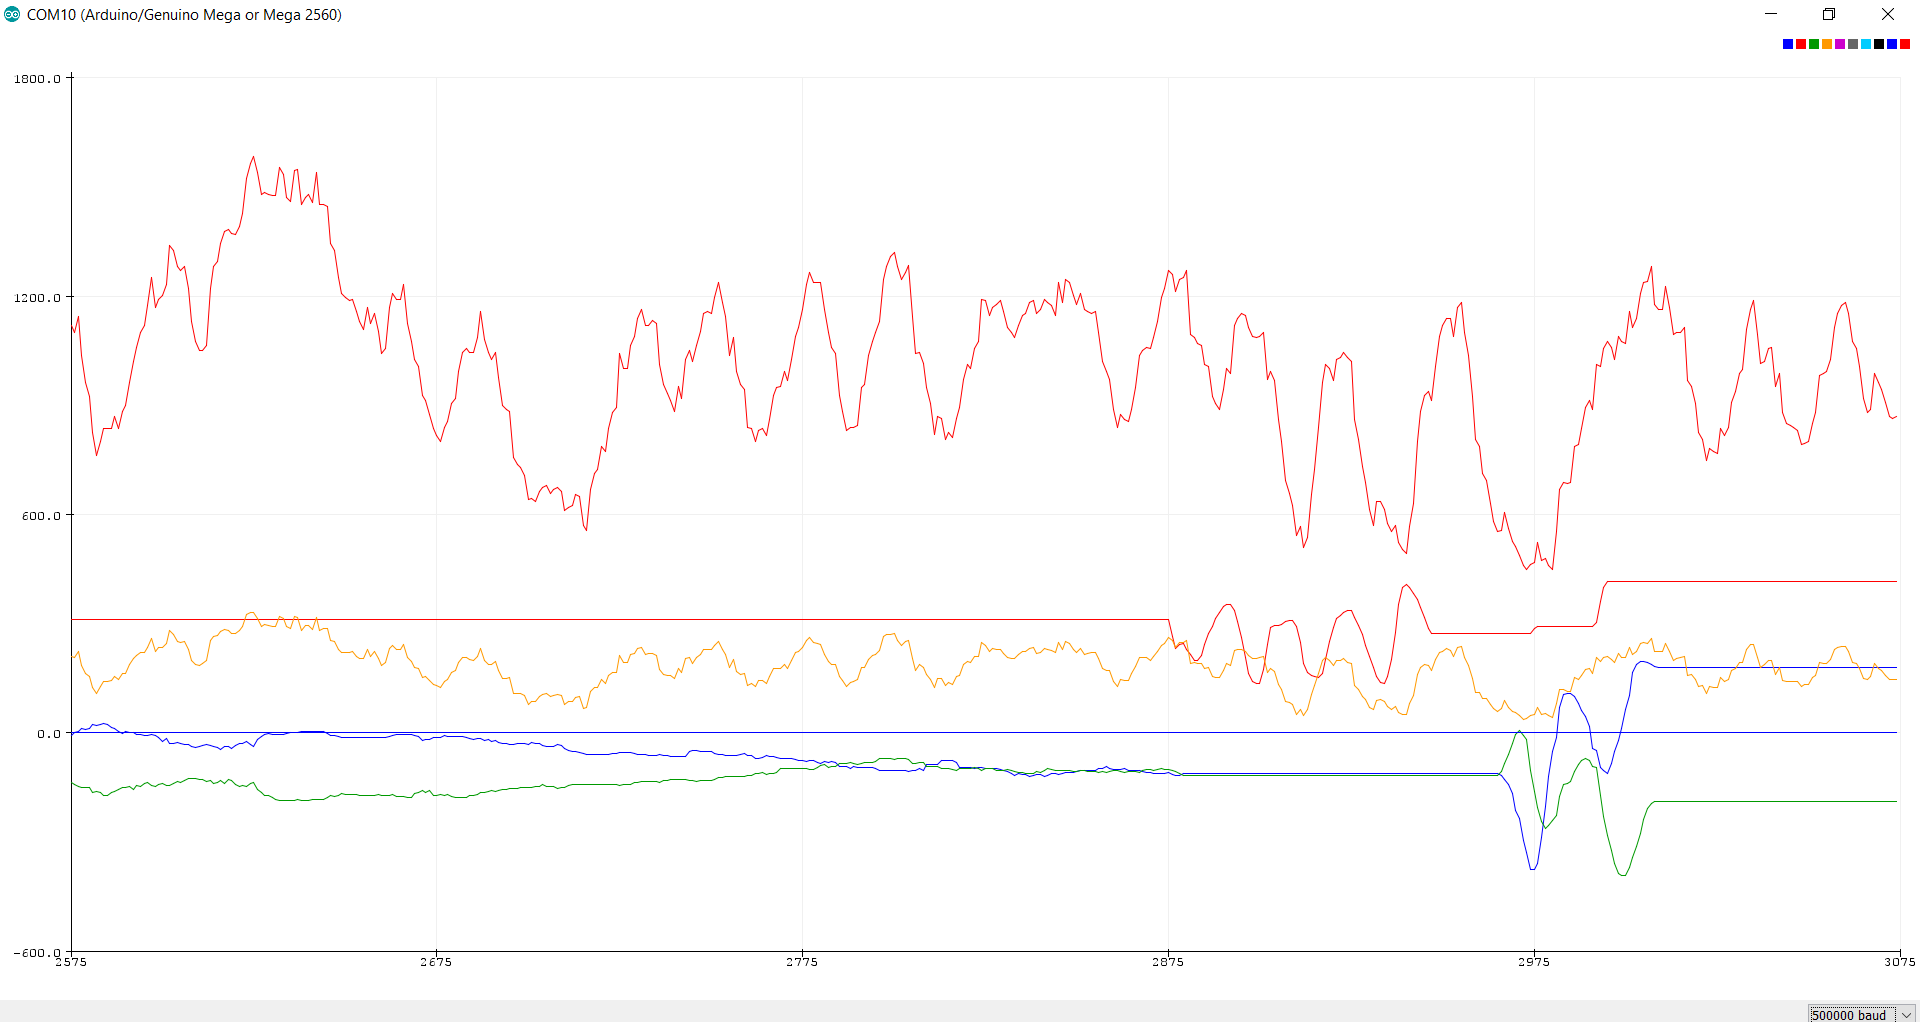
\includegraphics[width=12cm]{images/plotting.png}
    \caption{I2C Synchronization plotting with multiple devices.}
    \label{fig:plotting}
\end{figure}

When opening the description of each frame of a tiff files (can easily be done using Python scripts (\url{https://vidriotech.gitlab.io/scanimagetiffreader-python/}), you should see a line of String data separated by spaces and representing the signals values in the order they were transmitted.
You can also open the metadata of each .tiff files using FIJI (ImageJ) (see Figure \ref{fig:metadata}) but you will need additional libraries or python script to open the description of each frame inside the file (see Figure \ref{fig:description}).

\begin{figure}[h!]
    \centering
    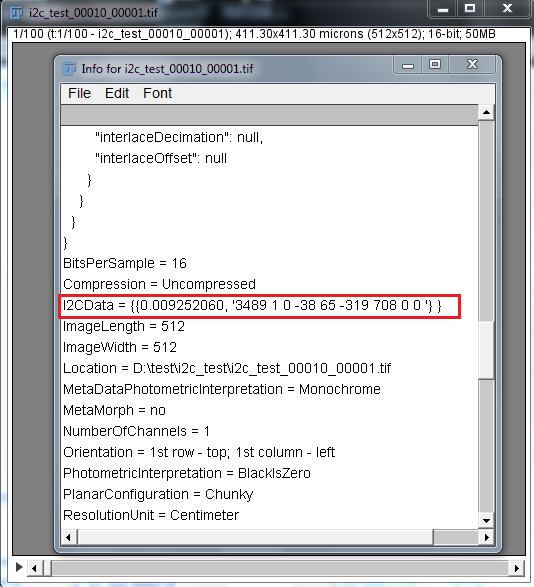
\includegraphics[width = 6cm]{images/metadata.png}
    \caption{Metadata as shown in "show Info" option in FIJI}
    \label{fig:metadata}
\end{figure}

\begin{figure}[h!]
    \centering
    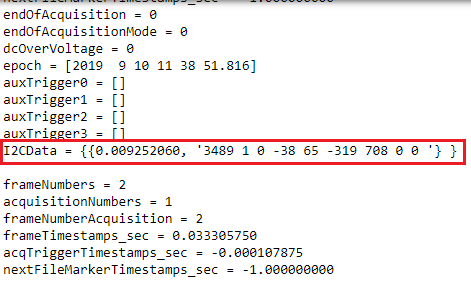
\includegraphics[width = 6cm]{images/description.png}
    \caption{Description for a specific frame of the file}
    \label{fig:description}
\end{figure}

A code snippet used to gather the description is shown in appendix \ref{codeDescription}.

\section{Troubleshooting}
\subsection{Nothing appears in the Serial plotter and Serial Monitor}
Check that the baud rate is set to 500 000.

\begin{figure}[h!b!t!]
    \centering
    
\includegraphics[width = 6cm]{images/baud.PNG}
    \caption{Set Baud rate to 500 000}
    \label{fig:baud}
\end{figure}

\subsection{Nothing plots on the Serial Plotter and the Serial monitor shows a growing single line of values}
You must end your last Serial printing by a "LF" character (line feed), being "\textbackslash n" or 0x0A in hex. Alternatively, you can also change your last print by: 
\begin{lstlisting}
Serial.print("yourData: "); Serial.println(yourData);
\end{lstlisting}

\subsection{Nothing plots on the Serial plotter and the Serial monitor shows "motion Sensor setup..." then nothing happens}
It is because the optical mice motion sensor are not plugged in or malfunctioning and the program awaits a response from them to continue.
Make sure to comment the line:
\begin{lstlisting}
#define MOTION_SENSOR
\end{lstlisting}
and then compile and upload the code if you are not using them.

\subsection{The plotting shows only a few signals and the rest are straight lines or very small}
The plotter does not automatically sets a scaling. Each value share the same axis. Therefore, a very low analog value or a digital value (highest value being 1) will appear extremely small or as a straight line in comparison.

Simply multiply the value (in the Serial.print() only !) by a relevant gain.

By default, the gain is set so that max values is 5000 (legacy from strain gauge 5V max value).

\subsection{I can't send I2C data}
Make sure that ScanImage is using the adress 0 as the I2C slave adress.
If not, you can change the slave adress in the code (either in integer or hex):
\begin{lstlisting}
Wire.beginTransmission(yourI2CSlaveAdressHere);
\end{lstlisting}


\subsection{My analog pins not connected read similar results to the other analog pins instead of reading zero}
If a pin has nothing connected to it, it will be floating and there is no reason to expect a reading of zero.

The Arduino Mega has only one ADC which will read the different analog pins using a multiplexer to connect the pin to the ADC. Moreover, this ADC uses a "hold\&sample" capacitor to read the pin by connecting to it, charging the capacitor, disconnecting the pin and then reading the voltage from the capacitor.
This means that when switching to an unconnected pin, the capacitor voltage will not change and the reading from the unconnected pin will be the same than the previous pin (albeit sometimes slightly lower due to capacitor discharging when reading the voltage).

To avoid it, either tie the unused pins to a pull-up or pull-down resistor (you can also do it using the integrated resistor of the Arduino chip) or comment the lines of code for reading the pins that are not connected (remember to compile and upload the code as well).\\

Note also that any wires connected to the pin will act as an antenna and is likely to pick up any stray capacitance from other wires, air, ... which will show when reading the pin if it is not driven by a strong signal (pull-up, pull-down, signal input).




\subsection{My new data doesn't appear on the plot}
Check that you plugged your signal in the correct pin. Also check that this pin is selected in the code as either digitalRead() or analogRead(). Just follow the guidelines in the code for each section (pin definition, data acquisition, plotting, I2C communication). The guidelines are written again here-below:

\begin{lstlisting}


/*TO ADD A NEW DATA:
   add the corresponding pin in the code:
      int myDataPin = "my pin number"

   add an acquisition value variable
      int myDataValue;

   add an I2C array to transmit this value.
   This array should have the size of the number of characters you want to send +1.
   i.e. to send 327, the array size is 4, because each char is one byte and we want to transmit bytes.
      int myDataI2cArray["my required size"];

   add the pinMode in Setup()
      pinMode(myDataPin, INPUT);

   in the acquisition part (dataAcquisition() function)
   add your data reading
    if it is a digital value:
      myDataValue = digitalRead(myDataPin)

    if it is an analog value:
      myDataValue = analogRead(myDataPin);


   add the value in plot:
       Serial.print("yourData: "); Serial.print(yourData); Serial.print(" ");
     Make sure that the last line of ArduinoPlotting is Serial.print(\n");

   add the data in the bytes conversion function i2cDataTransform
      ((String)myDataValue).toCharArray(myDataI2cArray, my array size);

   add the i2C communication line inbetween Wire.beginTransmission(0x00); and Wire.endTransmission();
      Wire.write(myDataI2cArray); Wire.write(" ");
*/
\end{lstlisting}


\newpage

\appendix

\section{Frame Description reading python script}
\label{codeDescription}
\lstinputlisting[language= Python]{PythonCode.txt}

%\section{C++ Main Code}
%\label{code}
%\lstinputlisting[language=C++]{180829_i2c_aurora206_V3.ino}




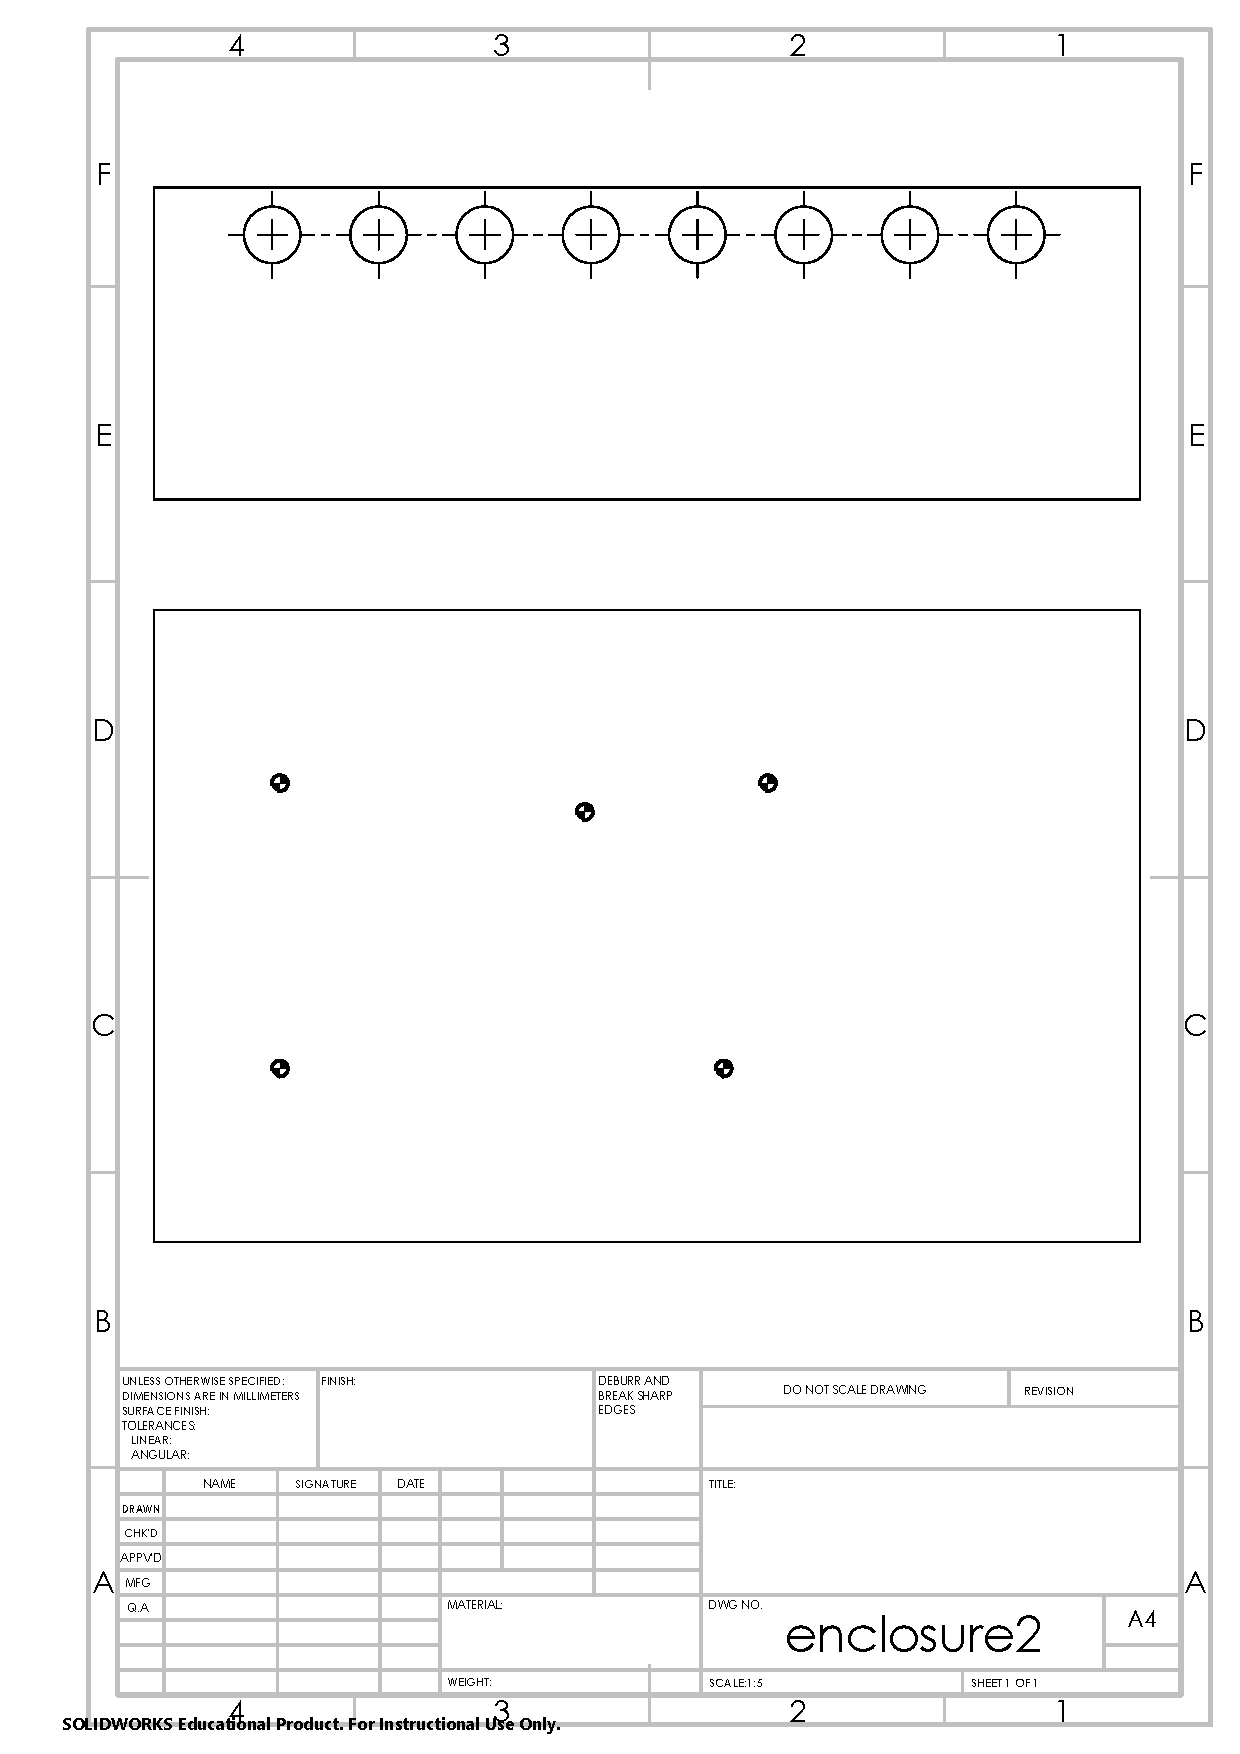
\includepdf[pagecommand= \section{Enclosure Plan 1 \label{plans}}, scale = 0.7, angle =0]{images/enclosureBiggerPlan1}

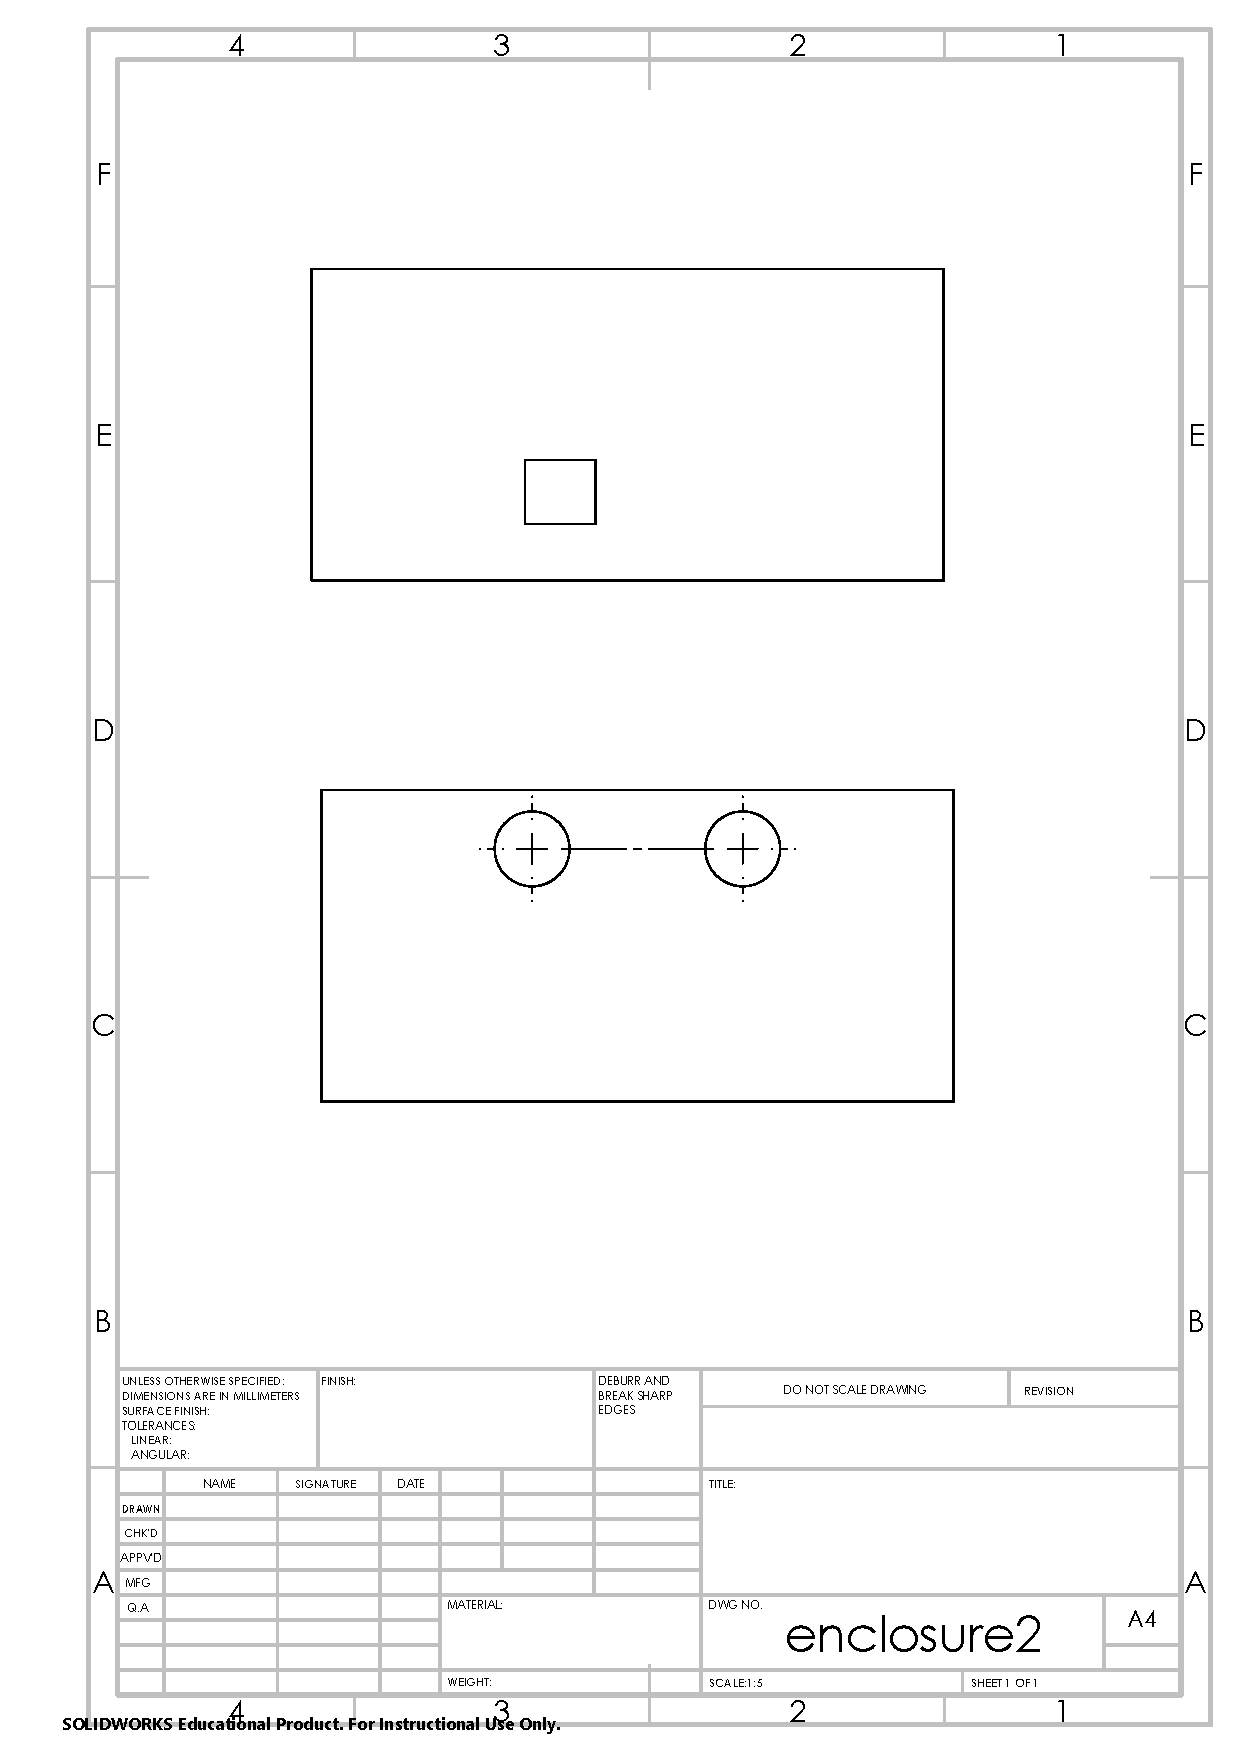
\includepdf[pagecommand= \section{Enclosure Plan 2}, scale = 0.7, angle =0]{images/enclosureBiggerPlan2}

\bibliographystyle{alpha}
\bibliography{biblio}

\end{document}